\documentclass[12pt]{scrreprt} % Set font size to 12pt

\usepackage{changepage} % Add the changepage package for the addmargin environment
\usepackage{blindtext} % Generate lorem ipsums
\usepackage{helvet} % Arial font (Arial is proprietary, so we use Helvetica instead)
\renewcommand{\familydefault}{\sfdefault}
\usepackage[margin=2.5cm]{geometry} % Set margins to 2.5cm on all sides
\usepackage{graphicx} % Add the graphicx package for including images
\usepackage{atbegshi} % Package for placing elements at absolute positions
\usepackage[allcolors=blue]{hyperref} % Add the hyperref package for hyperlinking
\usepackage{xcolor} % Add the xcolor package for color support
\usepackage{tabularx} % Add the tabularx package for advanced tables

\makeatletter
\def\@cite#1#2{$^{\mbox{\scriptsize [#1\if@tempswa , #2\fi]}}$}
\makeatother

% CONSIGNES POUR LA REDACTION DU RAPPORT DE PROJET

% CRITERES D'EVALUATION :
% Critères liés à votre travail et vos compétences :
% - Le respect des objectifs fixés
% - Les compétences techniques et scientifiques
% - L'aptitude à rechercher de l'information
% - L'implication et l'esprit d'initiative
%
% Critères liés à votre rapport de projet
% - La structuration du document
% - L'orthographe et l'expression écrite
% - Le descriptif de la mission
% - La valeur du contenu scientifique et technique
% - La précision des résumés en français, en anglais et la bibliographie
%
% Critères liés à votre soutenance
% - La qualité de la structuration et de l'expression
% - La qualité du diaporama
% - Le dynamisme et l'interactivité
% - La qualité des réponses, l'esprit critique sur le travail réalisé, qualité de la conclusion et des éventuelles perspectives.

% RAPPORT
% Informations générales
%
% Le rapport doit être rédigé par vos soins, en respectant les normes
% de rédaction indiquées ci-dessous. Il sera évalué sur la forme
% (orthographe, grammaire, ponctuation, langage approprié, etc.) et le fond
% (organisation, méthode, argumentation, etc.).
% Il devra avoir une longueur comprise entre 20 et 25 pages (hors annexes)
% et sera à rendre au format PDF.
% L'ensemble des comptes rendus hebdomadaires d'avancement constituera une rubrique annexe de votre rapport.
% Votre document doit comporter une bibliographie permettant d'identifier et de retrouver les documents cités.
%
% Le rapport est à remettre le 9 avril 2024.
%
% Format attendu du document
% - Police Arial
% - Taille des polices : Texte (12), Sections/Titres (14, gras)
% - Numérotation des sections : numérotation scientifique (1, 1.1, 1.1.1)
% - Numérotation des pages : centrale en bas de page
% - Numérotation des tableaux et des figures
% - Marges : 2,5 cm en haut, en bas, à gauche et à droite
% - Résumé (français) et abstract (anglais) sur la dernière page de couverture
% - La première et la quatrième de couverture doivent respecter scrupuleusement le modèle téléchargeable ci-après
% - La mise en page du corps du rapport est libre.




\begin{document}

% add the 0.jpg image to the top-left of the first page

\begin{titlepage}
    \newgeometry{left=1cm, right=1cm, top=1cm, bottom=1cm}

    \noindent
\includegraphics{0.jpg}
    
\includegraphics{1.jpg}
    \hfill
    
\includegraphics{2.jpg}
    \vspace{1cm}


    École Polytechnique de l'Université de Tours

    64, Avenue Jean

    Portalis 37200

    TOURS, FRANCE

    (33)2-47-36-14-14

    \href{http://www.polytech.univ-tours.fr}{\textcolor{red}{www.polytech.univ-tours.fr}}


    \vfill
    \begin{center}

        \Huge
        Parcours des écoles d'ingénieur Polytech
        \vspace{0.3cm}

        \textbf{Année 2023-2024}
        \vspace{0.5cm}


        \textbf{Projet Informatique : Labyrinthe}
    \end{center}
    \vfill

    % footer
    \begin{minipage}[t]{0.5\textwidth}
        \begin{flushleft}
            Étudiants
            \vspace{0.1cm}
            \hrule % horizontal
            \vspace{0.5cm}

            \textbf{Pacôme Renimel--Lamiré}
            \href{mailto:pacome.renimel--lamire@etu.univ-tours.fr}{\textcolor{blue}{pacome.renimel--lamire@etu.univ-tours.fr}}

            \textbf{Esteban Laurent}
            \href{mailto:esteban.laurent@etu.univ-tours.fr}{\textcolor{blue}{esteban.laurent@etu.univ-tours.fr}}
        \end{flushleft}
    \end{minipage}
    \begin{minipage}[t]{0.5\textwidth}
        \begin{flushright}
            Encadrant

            \vspace{0.1cm}
            \hrule % horizontal
            \vspace{0.5cm}

            \textbf{Christophe Lenté}

            \href{mailto:christophe.lente@univ-tours.fr}{\textcolor{blue}{christophe.lente@univ-tours.fr}}

        \end{flushright}
    \end{minipage}
\end{titlepage}
\restoregeometry


\chapter*{Avertissement}
\addcontentsline{toc}{chapter}{Avertissement} % Add the chapter to the table of contents

Ce document a été rédigé par Pacôme Renimel--Lamiré et Esteban Laurent susnommés les auteurs.

L’École Polytechnique de l’Université François Rabelais de Tours est représentée par Christophe Lenté susnommé le tuteur académique.

Par l’utilisation de ce modèle de document, l’ensemble des intervenants du projet acceptent les conditions définies ci-après.


Les auteurs reconnaissent assumer l’entière responsabilité du contenu du document ainsi que toutes suites judiciaires qui pourraient en découler du fait du non-respect des lois ou des droits d’auteur.

Les auteurs attestent que les propos du document sont sincères et assument l’entière responsabilité de la véracité des propos.

Les auteurs attestent ne pas s’approprier le travail d’autrui et que le document ne contient aucun plagiat.

Les auteurs attestent que le document ne contient aucun propos diffamatoire ou condamnable devant la loi.

Les auteurs reconnaissent qu’ils ne peuvent diffuser ce document en partie ou en intégralité sous quelque forme que ce soit sans l’accord préalable du tuteur académique et de l’entreprise.

Les auteurs autorisent l’école polytechnique de l’université François Rabelais de Tours à diffuser tout ou partie de ce document, sous quelque forme que ce soit, y compris après transformation en citant la source.

Cette diffusion devra se faire gracieusement et être accompagnée du présent avertissement.

\newpage
\renewcommand{\contentsname}{Table des matières} % Change the title of the table of contents to "Sommaire"
\tableofcontents


\newpage
\chapter*{Introduction}
\addcontentsline{toc}{chapter}{Introduction} % Add the chapter to the table of contents

% Ajouter un overview du projet
% Expliquer la motivation derrière le choix du sujet du projet : pourquoi est-ce important ? Quels sont les enjeux ?
% Décrire les buts et objectifs du projet
% Mentionner brièvement les algorithmes implémentés

Ce rapport a pour objectifs de décrire les différentes étapes de réalisation d'un programme informatique permettant de générer et résoudre automatiquement des labyrinthes, ainsi que de présenter les résultats obtenus.

L'objectif premier du projet consiste à créer un labyrinthe par une ou plusieurs méthodes différentes et à faire trouver à l'ordinateur un chemin menant vers la sortie. Pour ce faire, nous avons implémenté trois algorithmes différents :
\texttt{depth-first search}, \texttt{recursive backtracking} et \texttt{A*}.

La suite du projet a été laissée relativement libre, nous invitant à faire preuve d'imagination et de créativité pour aller au-delà des objectifs initiaux. Nous avons donc décidé d'ajouter des fonctionnalités supplémentaires, notamment un mode de jeu permettant à l'utilisateur d'évoluer dans des labyrinthes générés aléatoirement tout en étant poursuivi par des ennemis et en collectant des objets.

Nous avons également essayé de rendre notre programme le plus interactif possible, en rajoutant une interface graphique agréable et complète permettant de générer et résoudre des labyrinthes en personnalisant différents paramètres.

\paragraph{}

Afin de décrire de façon détaillée le déroulement de ce projet, ce rapport est divisé en plusieurs chapitres.

Dans un premier temps, nous étudierons brièvement un état de l'art des labyrinthes et des algorithmes de génération et de résolution de labyrinthes.

Nous expliquerons ensuite la méthodologie que nous avons appliquée pour mener à bien ce projet, en décrivant les différentes étapes de développement du programme.

Nous poursuivrons en présentant l'implémentation du programme, en décrivant la structure du code et les différents obstacles rencontrés.

Nous présenterons ensuite les résultats obtenus, en détaillant les performances du programme et les statistiques obtenues.

Enfin, nous prendrons du recul sur le projet en discutant de potentielles améliorations pouvant être apportées au projet à l'avenir, ainsi que de notre ressenti par rapport à ce que cette expérience a pu nous apporter.

\paragraph{}

Il peut être utile pour le correcteur de pouvoir tester le programme ou en consulter le code source au besoin avant, durant ou après la lecture de ce rapport. Pour ce faire, nous avons ajouté en annexe une section dédiée à l'installation du programme et à la consultation du code source.

\chapter{État de l'art et enjeux}


\section{Les labyrinthes : une fascination depuis l'Antiquité}

Selon le dictionnaire Larousse, un labyrinthe peut être défini comme suit :

"\textit{Dans l'Antiquité, [ il s'agissait d'un ] vaste édifice comprenant d'innombrables salles agencées de telle manière que l'on ne trouvait que difficilement l'issue.} \cite{LabyrintheLarousse}"

L'exemple le plus commun de labyrinthe associée à l'histoire humaine est probablement le labyrinthe de Crète, construit par Dédale pour emprisonner le Minotaure, un monstre mi-homme mi-taureau, au point que le mot dédale est rentré dans le langage courant pour désigner un lieu où l'on se perd facilement.

Toutefois, on retrouve des vestiges de tracés labyrinthiques depuis la fin de l'âge de bronze, la plus ancienne peuve de leur existence étant une tablette datant d'environ 1200 avant J.C. retrouvée à Pylos, en Grèce.\cite{Kern2000}

Les historiens s'accordent sur le fait que l'idée du labyrinthe était principalement symbolique, leur tracé n'étant quasiment jamais retrouvé à une échelle humaine, mais plutôt représenté de façon décorative sur des pièces de monnaie, des poteries, des bâtiments, etc.

De plus, le tracé le plus commun d'un labyrinthe, le labyrinthe unicursal, est un tracé continu sans embranchements, ce qui le rend impossible à résoudre de façon classique. Malgré le fait qu'il ne représente aucun intérêt récréatif, c'est celui qu'on retrouve le plus souvent dans les représentations de cette époque, ce qui montre bien la prévalence du symbolisme sur la fonctionnalité.

\begin{figure}[h]
    \centering
    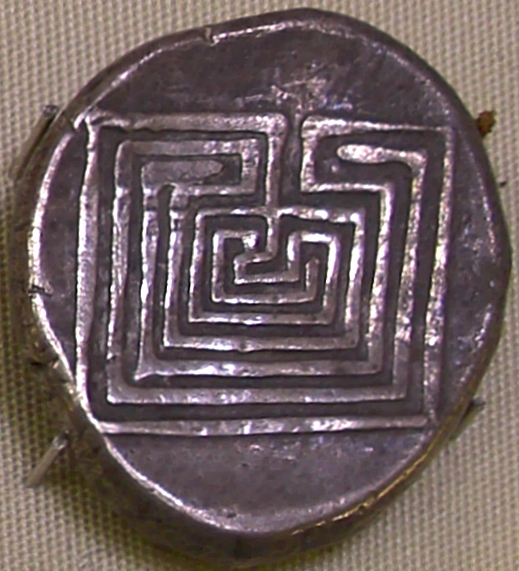
\includegraphics[width=0.3\textwidth]{images/pieceknossos.jpeg}
    \caption{Pièce d'argent représentant un labyrinthe unicursal, 400 avant J.C. - AlMare - CC-BY-SA-3}
\end{figure}

Ainsi, les labyrinthes que nous connaissons n'ont réellement fait leur apparition qu'au XVI\textsuperscript{e} siècle\cite{McCullough2004}, en tant que jeu de réflexion et de divertissement.

\section{Labyrinthes et informatique}

Aujourd'hui, on retrouve de nombreuses installations permettant d'évoluer dans des labyrinthes, souvent végétaux (Haies, Maïs, etc.). Le labyrinthe est devenu un symbole de réflexion, de concentration et de patience, et est souvent utilisé dans des jeux vidéos, des films, des livres, etc.

Cette notion a notamment pris une dimension toute particulière dans les domaines des mathématiques et plus tard, de l'informatique. En effet, un labyrinthe peut être vu comme un graphe, où chaque case est un nœud et chaque passage entre deux cases est une arête.

Ainsi, utiliser un labyrinthe est un excellent moyen d'en apprendre plus sur les algorithmes de recherche, qui sont indispensables à d'innombrables technologies que nous utilisons aujourd'hui : les jeux vidéos, les applications de navigation, les moteurs de recherche, les intelligences artificielles, etc.

De nombreux problèmes mathématiques bien connus sont d'ailleurs basés sur la théorie des graphes et donc sur les labyrinthes, comme le problème du cavalier (un cavalier doit visiter une unique fois chaque case d'un échiquier) ou celui des sept ponts de Königsberg, tous deux résolus par Euler dès le milieu du XVIII\textsuperscript{e} siècle\cite{Alexanderson2006}\cite{Euler1759}.

De la même façon que les labyrinthes ont été utilisés afin d'étudier la mémoire chez les rats, des compétitions de résolution de labyrinthes sont organisées chaque année, notamment par la société américaine \textit{Micromouse}, qui propose aux participants de créer un robot capable de résoudre un labyrinthe en un temps record, sans aucune connaissance préalable du tracé du labyrinthe.\cite{Veritasium2023}

\section{Algorithmes de génération et de résolution de labyrinthes}

\subsection{Génération de labyrinthes}

\subsubsection{Un peu de théorie}

Afin de générer un labyrinthe, il peut être très utile d'en apporter une définition mathématique plus rigoureuse.

Si on choisit l'approche de la théorie des graphes, alors un labyrinthe peut être décrit comme un graphe grille : un graphe non orienté où chaque nœud est relié à ses quatre voisins (haut, bas, gauche, droite) s'ils existent.

Chaque nœud représente un chemin du labyrinthe, et chaque arête représente le passage d'une case à une autre. Certaines propriétés intéressantes sont déjà présentes : on ne peut par exemple pas se déplacer d'une case à une autre si elles ne sont pas adjacentes, c'est à dire reliées par une arête.

Pour ajouter le concept de mur au labyrinthe, il suffit de retirer la connexion entre deux nœuds pour ajouter un "obstacle virtuel" entre les cases, empêchant ainsi le passage.

À partir de cette définition, on peut considérer que n'importe quel graphe ainsi dérivé d'un graphe grille, avec un nombre arbitraire d'arêtes manquantes, est un labyrinthe. Toutefois, afin de rendre les choses plus intéressantes, il est bon de rajouter quelques contraintes.

Il peut par exemple être intéressant de nécessiter l'existence d'au moins un chemin entre n'importe quelle case de départ, et n'importe quelle case d'arrivée. Cette contrainte est appelée la connexité du graphe, et est souvent utilisée pour garantir qu'un labyrinthe est "solvable".

On peut également pousser le vice et exiger que le chemin qui relie deux cases du labyrinthe soit unique. Si on considère notre graphe grille, alors un tel labyrinthe serait représenté par un arbre, c'est à dire un graphe convexe et acyclique (il est impossible de partir d'un sommet et d'y revenir sans rebrousser chemin au moins une fois). Plus encore, il s'agit d'un arbre couvrant, puisqu'il couvre l'ensemble des sommets du graphe de départ.

Dans ce contexte, un labyrinthe qui vérifie ces deux conditions est appelé un labyrinthe parfait. Ainsi, la plupart des algorithmes de génération ont été conçus pour produire des labyrinthes parfaits.

Toutefois, il est très souvent plus intéressant de travailler avec des labyrinthes non-parfaits, et où plusieurs chemins sont possibles. On peut ainsi tester les algorithmes de résolution sur un critère supplémentaire : la longueur du chemin trouvé, que l'on précisera dans la suite de cette partie.

Parallèlement, un algorithme de génération de labyrinthe peut être comparé sur la base de deux critères : le temps de génération, ainsi que la "difficulté" du labyrinthe généré, ce qui est assez peu objectif.

\subsubsection{L'algorithme "Depth-first search"}

Dans le cadre de ce projet, nous avons choisi de générer des labyrinthes en utilisant l'algorithme de \textit{depth-first search}, également appelé \textit{recursive backtracking}, un algorithme de type "diviser pour régner" qui consiste à diviser le problème en sous-problèmes plus petits, les résoudre, puis les combiner pour obtenir la solution du problème initial.

Malgré son nom, son implémentation ne nécéssite pas d'utiliser une récursion au sens strict, et est souvent plus performante de façon itérative, en utilisant une \textbf{pile} pour stocker les états précédents. L'utilisation d'une pile, en plus d'être plus sûre (en évitant d'éventuells erreurs liées à un manque de mémoire dans la pile d'appel des fonctions), permet de faciliter la visualisation de l'algorithme, en rendant accessibles toutes les données qui y sont liées à tout moment.

L'algorithme fonctionne de la façon suivante :

\begin{enumerate}
    \item On considère un labyrinthe où chaque case est entourée par des murs. On définit une pile vide.
    \item Choisir un point de départ dans le labyrinthe.
    \item Marquer ce point comme visité et l'ajouter à la pile.
    \item Tant qu'il existe des voisins non visités :
          \begin{enumerate}
              \item Retirer la case en haut de la pile et la définir comme la "case courante"
              \item Si la case courante possède au moins un voisin qui n'a pas été visité :
                    \begin{enumerate}
                        \item Ajouter la case courante à la pile
                        \item Choisir un de ses voisins non visités (aléatoirement)
                        \item Retirer le mur entre la case courante et le voisin choisi
                        \item Marquer le voisin comme visité et l'ajouter à la pile
                    \end{enumerate}
          \end{enumerate}
\end{enumerate}

Cet algorithme garantit la génération d'un labyrinthe parfait. De plus, il est relativement simple à implémenter et produit des labyrinthes avec une structure intéressante.

Après considération des alternatives existantes, nous avons jugé que l'intérêt d'implémenter d'autres algorithmes de génération de labyrinthes n'était pas suffisant pour justifier le temps et les ressources nécessaires à leur implémentation. En effet, les alternatives existantes telles que les algorithmes de Kruskal ou de Prim ne présentent pas d'avantages significatifs ou de résultats significativement différents par rapport à l'algorithme de \textit{depth-first search}.

La principale différence entre les labyrinthes générés par ces algorithmes réside dans sa structure : le \textit{depth-first search} génère des labyrinthes avec de longs couloirs, tandis que les algorithmes de Kruskal et de Prim génèrent des labyrinthes avec des couloirs plus courts, rendant une grande partie du labyrinthe fondamentalement inutile du point de vue de la résolution.

Afin d'ajouter de la diversité à nos labyrinthes, et de rendre le processus de résolution beaucoup plus intéressant, nous avons décider d'implémenter ce que nous avons appelé un "facteur de bouclage" : il s'agit d'un réel compris entre $0$ et $1$, et qui permet de transformer un labyrinthe parfait en labyrinthe comportant de nombreux chemins différents entre deux cases.

Une fois un labyrinthe généré, on sélectionne aléatoirement un certain nombre de murs en fonction du facteur de bouclage (un facteur de $0.5$ signifiant que la moitié des murs du labyrinthe seront retirés), et on les retire du labyrinthe. On obtient ainsi un labyrinthe non-parfait, mais toujours solvable.

\subsection{Résolution de labyrinthes}

\subsubsection{Un peu de théorie}

La résolution d'un labyrinthe est essentiellement un problème de recherche de chemin dans un graphe, mais appliqué à des graphes ayant des propriétés particulières, comme vu précédemment.

Ainsi, il est tout à fait possible d'utiliser n'importe quel algorithme de recherche de chemin dans un graphe pour résoudre n'importe quel labyrinthe, comme par exemple l'algorithme de Dijkstra.

Toutefois, le contexte du labyrinthe permet également de rajouter certaines contraintes optionnelles à la résolution, comme par exemple le fait de se mettre à la place d'un joueur ne pouvant pas voir l'ensemble du labyrinthe à la fois. De plus, certains algorithmes ne fonctionnent que sur des arbres couvrants, c'est à dire des labyrinthes parfaits.

On peut citer par exemple deux algorithmes triviaux de résolution de labyrinthes : le mur suiveur, qui consiste à suivre un mur à sa droite ou à sa gauche jusqu'à trouver la sortie, et celui de la "souris aléatoire", qui consiste à se déplacer aléatoirement dans le labyrinthe jusqu'à trouver la sortie.

Ce dernier algorithme est d'ailleurs plus intéressant qu'il en a l'air : il est évidemment très peu performant, mais c'est un exemple d'\textit{algorithme de Las Vegas}, c'est à dire un algorithme aléatoire qui est garanti de trouver une solution correcte au problème qui lui est présenté.

De son côté l'algorithme de mur suiveur fonctionne uniquement sur des labyrinthes parfaits, et peut rentrer dans des boucles infinies si ce n'est pas le cas.

Comme nos labyrinthes ne sont pas parfaits, et que l'objectif reste d'en trouver une solution dans un temps raisonnable, nous avons choisi d'implémenter deux algorithmes beaucoup plus performants que ceux-ci : \texttt{recursive backtracking} et \texttt{A*}.

\subsubsection{L'algorithme "Recursive backtracking"}

L'algorithme \texttt{recursive backtracking} est un algorithme qui consiste à identifier les impasses du labyrinthes, et de les "bannir" afin de ne plus les emprunter. Cet algorithme est bien le même que celui qui permet de générer des labyrinthes, mais en sens inverse. Il porte donc le même nom, mais afin d'éviter toute confusion, nous avons fait le choix de l'appeler exclusivement "\textit{recursive backtracking}", tandis que l'algorithme de génération est appelé "\textit{depth-first search}".

Bien que sur le papier, il soit similaire à celui que nous avons déjà étudié, il est en réalité légèrement différent dans son implémentation. En plus de la pile et de la liste de cases déjà visitées, on va également utiliser une liste de cases bannies, qui sont des cases qui ne mènent à aucune solution.

L'algorithme fonctionne de la façon suivante :

\begin{enumerate}
    \item On considère un labyrinthe quelconque, avec une case de départ et une case d'arrivée. On initialise une pile contenant la case de départ, une liste de cases déjà visitées vide, et une liste de cases bannies vide.
    \item Tant que la pile ne contient pas la case d'arrivée :
          \begin{enumerate}
              \item On choisit une case voisine non visitée, non bannie, et non séparée par un mur de la case en haut de la pile.
              \item Si aucune case n'est disponible, on retire la case en haut de la pile et on l'ajoute à la liste de cases bannies.
              \item Sinon, on ajoute la case choisie à la pile et on la marque comme visitée.
          \end{enumerate}

    \item Lorsque la pile contient la case d'arrivée, on a trouvé une solution : la pile contient le chemin entre la case de départ et la case d'arrivée.
\end{enumerate}

Cet algorithme est raisonnablement performant, mais n'est pas nécessairement garanti de trouver le chemin le plus court entre deux cases. Il est toutefois garanti de trouver une solution si elle existe.

\subsubsection{L'algorithme "A*"}

L'algorithme \texttt{A*} est un algorithme de recherche de chemin dans un graphe qui utilise une heuristique pour guider la recherche. Il est souvent utilisé dans des contextes où la recherche de chemin est difficile, comme par exemple dans les jeux vidéos, les applications de navigation, etc.

Une heuristique est une fonction qui permet de "guider" l'algorithme dans ses choix en faisant des hypothèses jugées "raisonnables". Par exemple, dans l'algorithme précédent, lorsque plusieurs cases sont valides, on en choisit une au hasard. Ici, on fera appel à une fonction qui permettra de choisir la case la plus "prometteuse" parmi les cases valides.

Cette fonction peut grandement varier en fonction du contexte, par exemple en tenant compte du poids d'une connexion dans un graphe (la vitesse de circulation sur une route par exemple). Ici, on utilisera la distance de Manhattan, c'est à dire la somme des distances horizontales et verticales entre deux cases.

Comme l'algorithme est basé sur des hypothèses, il n'est également pas garanti de trouver une solution optimale. Toutefois, il trouve généralement des solutions qui s'en approchent en un temps très court. De plus, il est garanti de trouver une solution si elle existe.

Ses nombreux avantages et sa grande adaptabilité en font un algorithme très populaire : il est notamment utilisé par défaut dans de nombreux moteurs de jeux vidéos, et est souvent utilisé dans des compétitions de résolution de labyrinthes.

\subsubsection{D'autres algorithmes}

Il existe de très nombreux autres algorithmes de résolution de labyrinthe, ayant tous leurs avantages et inconvénients. On peut citer par exemple l'algorithme de Dijkstra, l'algorithme de Bellman-Ford, l'algorithme de Floyd-Warshall, etc.

Bien que leur implémentation ne soit pas nécéssairement plus complexe que celle des algorithmes que nous avons choisi d'implémenter, nous avons préféré passer plus de temps à créer des visualisations et des fonctionnalités supplémentaires pour le programme plutôt que d'implémenter de nouveaux algorithmes.

L'ajout de ces algorithmes pourrait être une piste d'améliorations pour le futur, comme il le sera précisé dans le cinquième et dernier chapitre de ce rapport.

\chapter{Méthodologie}

Décrire les langages de programmation, librairies et outils utilisés (Python, Pygame-ce, Git, LaTeX, etc.)

Décrire les différentes étapes de développement du projet : conception, implémentation, tests, etc.

Peut être ne pas en faire un chapitre à part entière ?

\chapter{Implémentation}

Décrire la structure du programme

Expliquer comment le code est organisé, et comment les algorithmes sont implémentés

Décrire les différentes complications qui se sont présentées et la façon dont nous les avons résolu.

Ce sera probablement le chapitre le plus long

\chapter{Résultats}

Présenter les résultats obtenus

Ajouter des statistiques comme le temps de génération d'un labyrinthe, le nombre de nœuds explorés par A*, etc.

On peut aussi ajouter des statistiques sur les performances du programme, comme le temps d'exécution, la consommation de mémoire, etc, ainsi que sur le nombre de lignes, etc.

\chapter{Discussion et perspectives}

Interpréter les résultats obtenus et les comparer à ce qui était attendu

Analyser les avantages et inconvénients de chaque algorithme

Présenter ce que ce projet nous a permis d'apprendre

Proposer de potentielles améliorations qui pourraient être apportées à l'avenir



\chapter{Sandbox pour tester des trucs}


\chapter*{Conclusion}
\addcontentsline{toc}{chapter}{Conclusion} % Add the chapter to the table of contents

Résumer les points clés du projet

Réiterer sur le but de ce projet et ce que la recherche dans ce domaine permet d'apporter à la science

Donner son impression générale par rapport à ce que nous a apporté le projet

\newpage % Start a new page for the bibliography
\renewcommand{\bibname}{Bibliographie} % Change the title of the bibliography section to "Références"

\bibliographystyle{unsrt} % Set the bibliography style. Change "plain" to the style you want to use.
\bibliography{references} % Include the bibliography file. Change "references" to the name of your .bib file.
\addcontentsline{toc}{chapter}{Bibliographie} % Add the chapter to the table of contents

\chapter*{Compte rendus hebdomadaires}
\addcontentsline{toc}{chapter}{Compte rendus hebdomadaires} % Add the chapter to the table of contents

\chapter*{Annexes}
\addcontentsline{toc}{chapter}{Annexes} % Add the chapter to the table of contents

\section*{Annexe 1 : Code source et installation}
\addcontentsline{toc}{section}{Annexe 1 : Code source et installation} % Add the section to the table of contents

\subsection*{Prérequis}

Afin de pouvoir installer et exécuter le programme, il est nécessaire de disposer des éléments suivants :
\begin{enumerate}
    \item Python 3.10 ou supérieur. Les versions antérieures n'ont pas été testées et ne sont pas garantie de fonctionner.
    \item Des notions de base avec l'interface en ligne de commande de votre système d'exploitation.
\end{enumerate}

\subsection*{Installation}

Afin d'obtenir le code source du programme et l'installer sur votre machine, veuillez suivre les instructions suivantes (également décrites dans le fichier \texttt{README.md} du dépôt Git) :

\begin{enumerate}
    \item Télécharger le code source du programme en suivant l'une des trois méthodes suivantes :
          \begin{itemize}
              \item Cloner le dépôt Git à l'aide de la commande suivante :
                    \begin{verbatim}
git clone https://github.com/HerbeMalveillante/ProjetPeiP24.git      
              \end{verbatim}
              \item Télécharger le code source sous forme d'archive ZIP en cliquant sur le bouton "Code" du dépôt Git, puis sur "Download ZIP".
              \item Obtenir le code source à partir du fichier ZIP fourni avec ce rapport.
          \end{itemize}
    \item Ouvrir un terminal et se placer dans le dossier contenant le code source du programme.
    \item Vérifier la version de Python utilisée dans le PATH à l'aide de la commande suivante :
          \begin{verbatim}
python --version
    \end{verbatim}
    \item (optionnel) Créer un environnement virtuel Python à l'aide de la commande suivante :
          \begin{verbatim}
python3 -m venv .envi

# activer l'environnement virtuel sur Unix
source .envi/bin/activate

# activer l'environnement virtuel sur Windows
.envi\Scripts\activate
    \end{verbatim}
    \item Installer les dépendances du programme à l'aide de la commande suivante :
          \begin{verbatim}
python3 -m pip install --upgrade pip
python3 -m pip install -r requirements.txt
    \end{verbatim}
          Veuillez noter que si une erreur liée à Pygame survient, il convient de vérifier que la version installée est bien la version "communauté" de Pygame (\texttt{pygame-ce}), et non la version officielle (\texttt{pygame}).

    \item Lancer le programme à l'aide de la commande suivante :
          \begin{verbatim}
python3 main.py
    \end{verbatim}

\end{enumerate}



\newpage

\begin{center}
    \Huge
    Projet Informatique : Labyrinthe
\end{center}

\section*{Résumé}

\blindtext

\section*{Mots-clés}

Labyrinthe, ajouter, d'autres, mots, clés

\section*{Abstract}
\blindtext

\section*{Keywords}

Labyrinth, add, other, keywords

\hrulefill

\vfill

\newcolumntype{Y}{>{\raggedleft\arraybackslash}X} % Redefine the X column type to align the text to the right

\begin{table}[h]
    \begin{tabularx}{\textwidth}{|X|Y|}
        \hline
        Encadrant académique              & Étudiants                               \\
        \textcolor{red}{Christophe Lenté} & \textcolor{red}{Pacôme Renimel--Lamiré} \\
                                          & \textcolor{red}{Esteban Laurent}        \\
        \hline
    \end{tabularx}
\end{table}



\end{document}